\section{Definiciones y ejemplos}

\subsection{}

{\nologo
\begin{frame}\frametitle{Funciones}

\vspace{-3mm}

\begin{block}{\textbf{Definición 1 (Función)}}
	\justifying
	Una \textbf{función} $f$ de un conjunto $D$ en un conjunto $E$ es una correspondencia que asigna a \underline{todo} elemento $x$ de $D$, 
	\underline{exactamente} un elemento $y$ de $E$.
	
	\vspace{-5mm}
	
	\begin{columns}
		\hspace{5mm}
		\begin{column}{0.5\textwidth}
			% \vspace{-1cm}
			\begin{figure}[H]
				\centering
				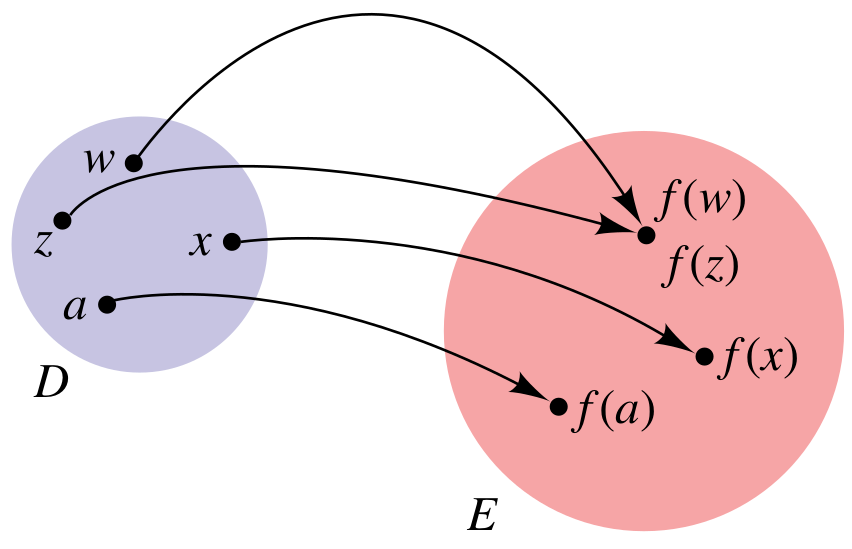
\includegraphics[width=4cm]{imagenes/funcion1}
				% .: 0x0 pixel, 0dpi, 0.00x0.00 cm, bb=
				%  \caption{Las flechas indican que}
			\end{figure}   
		\end{column}
		% \hspace{-5mm}
		\begin{column}{0.4\textwidth}  %%<--- here
			% \vspace{-2mm}
			\begin{figure}[H]
				\centering
				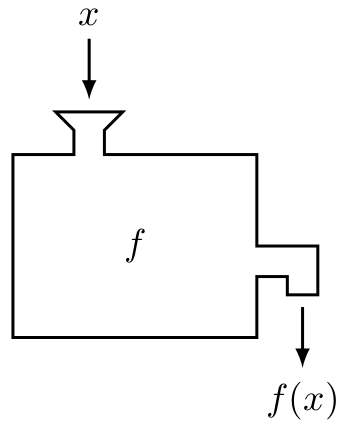
\includegraphics[width=2cm]{imagenes/funcion2}
				% .: 0x0 pixel, 0dpi, 0.00x0.00 cm, bb=
				%  \caption{Las flechas indican que}
			\end{figure}   
		\end{column}
	\end{columns}
	
	% \vspace{-1mm}
	% \begin{figure}[H]
	%  \centering
	%  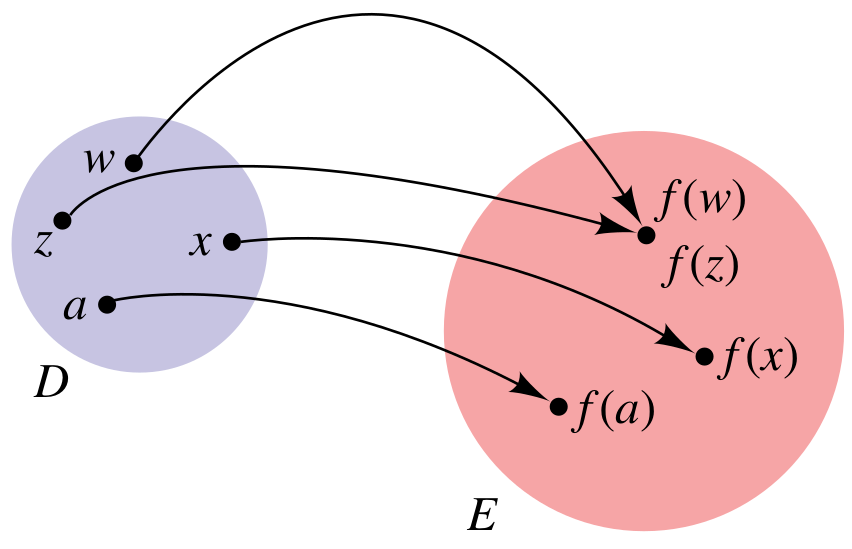
\includegraphics[width=4cm]{imagenes/funcion1}
	% \end{figure}   
\end{block}

\vspace{-0mm}

%\begin{alertblock}{\textbf{Observación 1}}
%	\begin{enumerate}
%		\item[\labelname{$a$}] El elemento $x$ de $D$ es el \textbf{argumento} de $f$.
%		\item[\labelname{$b$}] El conjunto $D$ es el \textbf{dominio} de la función.
%		\item[\labelname{$c$}] El elemento $y$ de $E$ es el valor de $f$ en $x$ o \textbf{imagen} de $x$ bajo $f$.
%		\item[\labelname{$d$}] La \textbf{imagen} de $x$ bajo $f$ se denota por $f(x)$ y se lee ``$f$ de $x$''.
%		\item[\labelname{$e$}] El rango de $f$ es el subconjunto de $E$ formado por todos las imágenes $f(x)$ para $x$ en $D$.
%		%  \item Si $f$ es una función de $D$ en $E$, escribimos $f:D\to E$.
%	\end{enumerate}
%\end{alertblock}

\vspace{-1mm}

\begin{alertblock}{\textbf{Observación 1}}
	\begin{enumerate}
		\item[\labelname{$a$}] Una función $f$ de $D$ en $E$ se denota por $f:D \to E$.
		\item[\labelname{$b$}] El conjunto $D$ es el \textbf{dominio} de la función.
		\item[\labelname{$c$}] El conjunto $E$ es el \textbf{codominio} de la función.
		\item[\labelname{$d$}] El elemento $y=f(x)$ de $E$ se llama \textbf{imagen} de $x$ bajo $f$.
		\item[\labelname{$e$}] La preimagen de $y$ en $E$ es el conjunto de todos los $x$ en $D$ tales que $f(x)=y$.
%		\item[\labelname{$e$}] La \textbf{imagen} de $f$ es el subconjunto de $E$ formado por todos las imágenes $f(x)$ para $x$ en $D$.
	\end{enumerate}
\end{alertblock}

\end{frame}
}

% ---------------------------------------------------------------------------------------------------

\subsection{}

{\nologo
\begin{frame}%\frametitle{Ejemplos}

\begin{block}{\textbf{Definición 1 (Función)}}
	\justifying
	Una \textbf{función} $f$ de un conjunto $D$ en un conjunto $E$ es una correspondencia que asigna a \underline{todo} elemento $x$ de $D$, 
	\underline{exactamente} un elemento $y$ de $E$.
	
	\vspace{-5mm}
	
	\begin{columns}
		\hspace{5mm}
		\begin{column}{0.5\textwidth}
			% \vspace{-1cm}
			\begin{figure}[H]
				\centering
				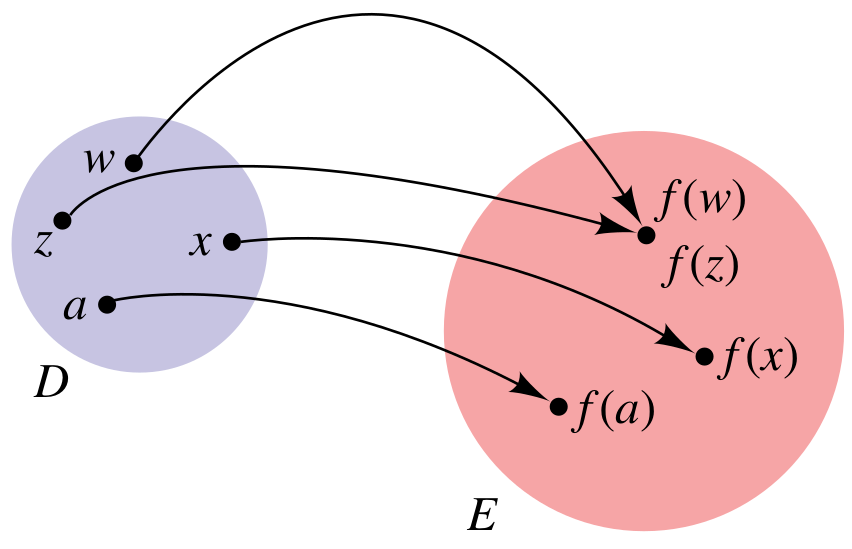
\includegraphics[width=4cm]{imagenes/funcion1}
				% .: 0x0 pixel, 0dpi, 0.00x0.00 cm, bb=
				%  \caption{Las flechas indican que}
			\end{figure}   
		\end{column}
		% \hspace{-5mm}
		\begin{column}{0.4\textwidth}  %%<--- here
			% \vspace{-2mm}
			\begin{figure}[H]
				\centering
				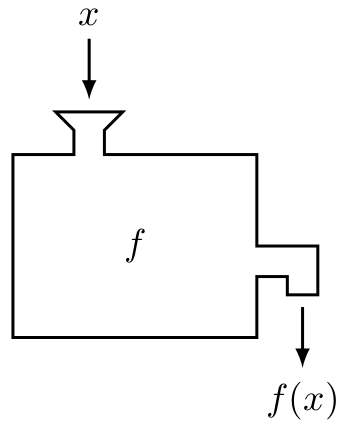
\includegraphics[width=2cm]{imagenes/funcion2}
				% .: 0x0 pixel, 0dpi, 0.00x0.00 cm, bb=
				%  \caption{Las flechas indican que}
			\end{figure}   
		\end{column}
	\end{columns}
	
	% \vspace{-1mm}
	% \begin{figure}[H]
	%  \centering
	%  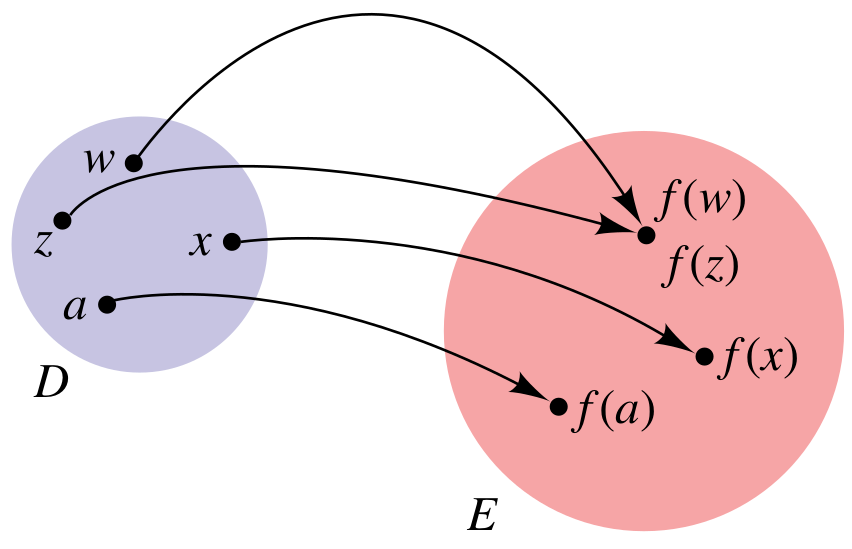
\includegraphics[width=4cm]{imagenes/funcion1}
	% \end{figure}   
\end{block}

%\begin{problock}{\textbf{Ejemplo 1.1.}}
%	\justifying
%	Sea $f$ la función con dominio $\r$ definida por $f(x)=x^2$ para cada $x$ en $\r$.
%	\begin{enumerate}
%		\item[\labelname{$a$}] Halle $f(-6), f(\sqrt{3}), f(a+b), f(a)+ f(b)$
%		\item[\labelname{$b$}] Halle el rango de $f$.
%	\end{enumerate}
%\end{problock}

\begin{ej}{\textbf{Ejemplo 1}}
	\justifying
	Sea $f$ la función con dominio $\r$ definida por $f(x)=x^2$ para cada $x$ en $\r$.
	\begin{enumerate}
		\item[\labelname{$a$}] Halle $f(-6), f(\sqrt{3}), f(a+b), f(a)+ f(b)$
		\item[\labelname{$b$}] Halle el rango de $f$.
	\end{enumerate}
\end{ej}
\textit{Solución.}

\end{frame}
}

% ---------------------------------------------------------------------------------------------------

\subsection{}

\begin{frame}[c]\frametitle{Funciones entre espacios vectoriales}

\begin{alertblock}{\textbf{Observación 2}}
	Vamos a considerar funciones 
	\[
		T:V \to W
	\]
	donde $V$ y $W$ son espacios vectoriales.
\end{alertblock}


\end{frame}

% ---------------------------------------------------------------------------------------------------

\subsection{}

\begin{frame}\frametitle{Funciones entre espacios vectoriales}
	
	\begin{ej}{\textbf{Ejemplo 2}}
		\justifying
		Considere la función $T:\r^2\to \r^2$ definida por 
		\[
		T(v_1,v_2) = (v_1-v_2, v_1+2v_2).
		\]
		
		\vspace{-2mm}
		\begin{enumerate}
			\item[\labelname{$a$}] Encuentre la imagen de $\mathbf{v}=(1,2)$.
			\item[\labelname{$b$}] Encuentre la preimagen de $\mathbf{w}=(-1,11)$.
		\end{enumerate}
	\end{ej}
	\textit{Solución.}
	
\end{frame}

% ---------------------------------------------------------------------------------------------------

\subsection{}

{\nologo
\begin{frame}\frametitle{Transformaciones lineales}

\begin{defi}{\textbf{Definición 2 (Transformación lineal)}}\justifying
	Sean $V$ y $W$ espacios vectoriales y $T:V\to W$ una función. Se dice que $T$ es una \textbf{\textit{transformación lineal}}
	si para todo vector $\mathbf{u}$ y $\mathbf{v}$ en $V$ y todo escalar $c$ se cumplen las siguientes propiedades:
	\begin{enumerate}
		\item[\labelname{$a$}] $T(\mathbf{u} + \mathbf{v}) = T(\mathbf{u}) + T(\mathbf{v})$
		\item[\labelname{$b$}] $T(c \mathbf{u}) = c\, T(\mathbf{u})$
	\end{enumerate}
\end{defi}	

\begin{alertblock}{\textbf{Observación 3}}
	\begin{center}
		\tikzstyle{mybox} = [draw=blue, fill=blue!10, very thick,
		rectangle, rounded corners, inner sep=5pt, inner ysep=5pt]
		\tikzstyle{fancytitle} =[fill=red, text=white]	
		\begin{tikzpicture}[thick,scale=0.8, every node/.style={scale=1}]%[scale=.8,font=\scriptsize]
		\draw[help lines,white,dotted] (0,-1) grid (13,3);	
		% Suma
		\fill[color=black,draw] (0,0) node[above, right] {\Large $T(\mathbf{u} \ + \ \mathbf{v}) \ = \ T(\mathbf{u}) \ + \ T(\mathbf{v})$};
		\node[draw] at (1.45,2) [mybox] (box){%
			\begin{minipage}{0.07\textwidth}
			Suma en $V$
			\end{minipage}	
		};
		\draw [line width=0.5mm,color=blue,->] (1.45,1.4) -- (1.45,0.3);
		\node[draw] at (4.82,2) [mybox] (box){%
			\begin{minipage}{0.075\textwidth}
			Suma en $W$
			\end{minipage}	
		};
		\draw [line width=0.5mm,color=blue,->] (4.82,1.4) -- (4.82,0.3);
		% Producto por escalar
		\fill[color=black,draw] (8,0) node[above, right] {\Large $T(c\mathbf{u}) \hspace{4mm} = \hspace{4mm} c\ T(\mathbf{u})$};
		\node[draw] at (8.9,2) [mybox] (box){%
			\begin{minipage}{0.115\textwidth}
			\justifying Producto en $V$
			\end{minipage}	
		};
		\draw [line width=0.5mm,color=blue,->] (8.9,1.4) -- (8.9,0.3);	
		\node[draw] at (11.3,2) [mybox] (box){%
			\begin{minipage}{0.115\textwidth}
			\justifying Producto en $W$
			\end{minipage}	
		};
		\draw [line width=0.5mm,color=blue,->] (11.3,1.4) -- (11.3,0.3);	
		\end{tikzpicture}
	\end{center}
\end{alertblock}

\end{frame}
}

% ---------------------------------------------------------------------------------------------------

\subsection{}

\begin{frame}\frametitle{Transformaciones lineales}

%\begin{defi}{\textbf{Definición 2 (Transformación lineal)}}\justifying
%	Sean $V$ y $W$ espacios vectoriales y $T:V\to W$ una función. Se dice que $T$ es una \textbf{\textit{transformación lineal}}
%	si para todo vector $\mathbf{u}$ y $\mathbf{v}$ en $V$ y todo escalar $c$ se cumplen las siguientes propiedades:
%	\begin{enumerate}
%		\item[\labelname{$a$}] $T(\mathbf{u} + \mathbf{v}) = T(\mathbf{u}) + T(\mathbf{v})$
%		\item[\labelname{$b$}] $T(c \mathbf{u}) = c\, T(\mathbf{u})$
%	\end{enumerate}
%\end{defi}	

\begin{ej}{\textbf{Ejemplo 3}}
	\justifying
	Muestre que la función $T:\r^2\to \r^2$ definida por 
	\[
	T(v_1,v_2) = (v_1-v_2, v_1+2v_2)
	\]
	es una tranformación lineal.
\end{ej}
\textit{Solución.}

\end{frame}

% ---------------------------------------------------------------------------------------------------

\subsection{}

\begin{frame}\frametitle{Funciones que no son transformaciones lineales}

%\begin{defi}{\textbf{Definición 2 (Transformación lineal)}}\justifying
%	Sean $V$ y $W$ espacios vectoriales y $T:V\to W$ una función. Se dice que $T$ es una \textbf{\textit{transformación lineal}}
%	si para todo vector $\mathbf{u}$ y $\mathbf{v}$ en $V$ y todo escalar $c$ se cumplen las siguientes propiedades:
%	\begin{enumerate}
%		\item[\labelname{$a$}] $T(\mathbf{u} + \mathbf{v}) = T(\mathbf{u}) + T(\mathbf{v})$
%		\item[\labelname{$b$}] $T(c \mathbf{u}) = c\, T(\mathbf{u})$
%	\end{enumerate}
%\end{defi}	

\begin{ej}{\textbf{Ejemplo 4}}
	\justifying
	Muestre que las siguientes funciones \textbf{no} son transformaciones lineales.
	\begin{enumerate}
		\item[\labelname{$a$}] $f:\r\to \r$ definida por $f(x)=2x+1$.
		\item[\labelname{$b$}] $g:\r\to \r$ definida por $g(x)=x^2$.
		\item[\labelname{$c$}] $h:\r\to \r$ definida por $h(x)=\sen x$.
	\end{enumerate}
\end{ej}
\textit{Solución.}

\end{frame}

% ---------------------------------------------------------------------------------------------------

\subsection{}

\begin{frame}\frametitle{Transformaciones lineales cero e identidad}

\begin{defi}{\textbf{Definición 3 }}\justifying
	Sean $V$ y $W$ espacios vectoriales.
	\begin{enumerate}
		\item[\labelname{$a$}] La \textbf{\textit{transformación cero}} es la función $T:V\to W$ definida por
		\[
			T(\mathbf{v}) = \mathbf{0}_{\scalebox{0.4}{W}}, \quad \text{ para todo } \mathbf{v} \text{ en } V.
		\]
		\item[\labelname{$b$}] La \textbf{\textit{transformación identidad}} es la función $T:V\to V$ definida por
		\[
		T(\mathbf{v}) = \mathbf{v}, \quad \text{ para todo } \mathbf{v} \text{ en } V.
		\]
	\end{enumerate}
\end{defi}	

\begin{prop}{\textbf{Propiedad 1}}
	\justifying
	La \textbf{\textit{transformación cero}} y la \textbf{\textit{transformación identidad}} son transformaciones lineales.
\end{prop}	

\end{frame}

% ---------------------------------------------------------------------------------------------------

\subsection{}

\begin{frame}\frametitle{Propiedades de las transformaciones lineales}
	
	\begin{prop}{\textbf{Propiedad 2}}
		\justifying
		Sea $T:V\to W$ una transformación lineal y suponga que $\mathbf{u}$ y $\mathbf{v}$ son vectores en $V$.
		Entonces:
		\begin{enumerate}
			\item[\labelname{$a$}] $T(\mathbf{0}_{\scalebox{0.4}{V}})=\mathbf{0}_{\scalebox{0.4}{W}}$.
			\item[\labelname{$b$}] $T(-\mathbf{v})=-T(\mathbf{v})$.
			\item[\labelname{$c$}] $T(\mathbf{u}-\mathbf{v})=T(\mathbf{u})-T(\mathbf{v})$.
			\item[\labelname{$d$}] Si $\mathbf{v} = c_1\mathbf{v}_1 + c_2\mathbf{v}_2 + \cdots c_n\mathbf{v}_n$, entonces
			\[
			T(\mathbf{v}) =  c_1T(\mathbf{v}_1) + c_2T(\mathbf{v}_2) + \cdots + c_nT(\mathbf{v}_n)
			\]
		\end{enumerate}
	\end{prop}	
		
	
\end{frame}


% ---------------------------------------------------------------------------------------------------

\subsection{}

\begin{frame}\frametitle{Propiedades de las transformaciones lineales}


\begin{ej}{\textbf{Ejemplo 5}}
	\justifying
	Sea $T:\r^3\to \r^3$ una transformación lineal tal que 
	\[
		\begin{array}{r@{\hspace{0.6\tabcolsep}}c@{\hspace{0.6\tabcolsep}}l}
			T(1,0,0) & = & (2,-1,4) \\[2mm]
			T(0,1,0) & = & (1,5,-2) \\[2mm]
			T(0,0,1) & = & (0,3,1) 
		\end{array}
	\]
	
	\vspace{-1mm}
	Calcule $T(2,3,-2)$.
\end{ej}
\textit{Solución.}

\end{frame}

% ---------------------------------------------------------------------------------------------------

\subsection{}

\begin{frame}\frametitle{Transformación lineal definida por una matriz}

\begin{ej}{\textbf{Ejemplo 6}}
	\justifying
	Considere la función $T:\r^2\to \r^3$ definida por
	\[
	T(\mathbf{v}) = A\mathbf{v} = 
	\left(
	\begin{array}{@{\hspace{0.3\tabcolsep}}r@{\hspace{1.2\tabcolsep}}r@{\hspace{0.3\tabcolsep}}}
		 3 & 0 \\[1mm]
		 2 & 1 \\[1mm]
		-1 & -2 
	\end{array}
	\right)
	\left(
	\begin{array}{@{\hspace{0.3\tabcolsep}}c@{\hspace{0.3\tabcolsep}}}
	v_1 \\[2mm]
	v_2
	\end{array}
	\right).
	\]
	
%	\vspace{-1mm}
	\begin{enumerate}
		\item[\labelname{$a$}] Calcule $T(2,-1)$.
		\item[\labelname{$b$}] Muestre que $T$ es una transformación lineal.
	\end{enumerate}	
\end{ej}
\textit{Solución.}

\end{frame}

% ---------------------------------------------------------------------------------------------------

\subsection{}

{\nologo
\begin{frame}\frametitle{Transformaciones lineales definidas por una matrices}

\begin{prop}{\textbf{Propiedad 2}}
	\justifying
	Sea $A$ una matriz $m\times n$. La función $T$ definida por
	\[
		T(\mathbf{v}) = A\mathbf{v}
	\]
	es una transformación lineal de $\r^n$ en $\r^m$.

\end{prop}	

\begin{alertblock}{\textbf{Observación 3}}
	\[
	A\mathbf{v} = 
	\left(
	\begin{array}{@{\hspace{0.3\tabcolsep}}c@{\hspace{\tabcolsep}}c@{\hspace{\tabcolsep}}c@{\hspace{\tabcolsep}}c@{\hspace{0.3\tabcolsep}}}
	a_{11} & a_{12} & \cdots & a_{1n} \\[1mm]
	a_{21} & a_{22} & \cdots & a_{2n} \\[1mm]
	\vdots & \vdots &        & \vdots \\[1mm]
	a_{m1} & a_{m2} & \cdots & a_{mn} 
	\end{array}
	\right)
	\hspace{-3mm}
	\underbrace{
	\left(
	\begin{array}{@{\hspace{0.3\tabcolsep}}c@{\hspace{0.3\tabcolsep}}}
	v_1 \\[2mm]
	v_2 \\[2mm]
	\vdots \\[2mm]
	v_n
	\end{array}
	\right)
	}_{\text{vector en } \r^n}
	\hspace{-2mm} = \hspace{0mm}
	\underbrace{
	\left(
	\begin{array}{@{\hspace{0.1\tabcolsep}}c@{\hspace{0.1\tabcolsep}}}
	a_{11}v_1 + a_{12}v_2  + \cdots + a_{1n}v_n \\[2mm]
	a_{21}v_1 + a_{22}v_2  + \cdots + a_{2n}v_n \\[2mm]
	\vdots \\[2mm]
	a_{m1}v_1 + a_{m2}v_2  + \cdots + a_{mn}v_n \\[2mm]
	\end{array}
	\right)
	}_{\text{vector en } \r^m}
	\]
\end{alertblock}

\end{frame}
}

% ---------------------------------------------------------------------------------------------------

\subsection{}

\begin{frame}\frametitle{Rotación en el plano}

\begin{ej}{\textbf{Ejemplo 7}}
	\justifying
	Muestre que la transformación lineal  $T:\r^2\to \r^2$ definida por la matriz
	\[
	A = 
	\left(
	\begin{array}{@{\hspace{0.3\tabcolsep}}r@{\hspace{1.2\tabcolsep}}r@{\hspace{0.3\tabcolsep}}}
	\cos\theta & -\sen\theta \\[1mm]
	\sen\theta & \cos\theta 
	\end{array}
	\right)
	\]
	tiene la propiedad de rotar todo vector en $\r^2$, un ángulo $\theta$ en sentido contrario a las
	manecillas del reloj.
	
\end{ej}
\textit{Solución.}

\end{frame}

% ---------------------------------------------------------------------------------------------------

\subsection{}

\begin{frame}\frametitle{Proyección en $\r^3$}

\begin{ej}{\textbf{Ejemplo 8}}
	\justifying
	Considere la transformación lineal  $T:\r^3\to \r^3$ definida por la matriz
	\[
	A = 
	\left(
	\begin{array}{@{\hspace{0.3\tabcolsep}}c@{\hspace{1.6\tabcolsep}}c@{\hspace{1.6\tabcolsep}}c@{\hspace{0.3\tabcolsep}}}
	1 & 0 & 0 \\[1mm]
	0 & 1 & 0 \\[1mm]
	0 & 0 & 0 
	\end{array}
	\right).
	\]
	Analice cómo transforma $T$ a todo vector en $\r^3$.
	
\end{ej}
\textit{Solución.}

\end{frame}

% ---------------------------------------------------------------------------------------------------

\subsection{}

\begin{frame}\frametitle{Transformación lineal entre espacios de matrices}

\begin{ej}{\textbf{Ejemplo 9}}
	\justifying
	Muestre que la función  $T:M_{mn}\to M_{nm}$ definida por 
	\[
		T(A) = A^T.
	\]
	es una transformación lineal.
	
\end{ej}
\textit{Solución.}

\end{frame}

% ---------------------------------------------------------------------------------------------------

\subsection{}

\begin{frame}\frametitle{El operador de multiplicación}
	
	\begin{ej}{\textbf{Ejemplo 10}}
		\justifying
		Demuestre que la función  $T:P_2\to P_3$ definida por 
		\[
		(Tp)(x) = xp(x)
		\]
		es una transformación lineal.
		
	\end{ej}
	
\end{frame}

% ---------------------------------------------------------------------------------------------------

\subsection{}

\begin{frame}\frametitle{El operador diferencial (cálculo)}

\begin{ej}{\textbf{Ejemplo 11}}
	\justifying
	Muestre que la función  $D:C^1[a,b]\to C^1[a,b]$ definida por 
	\[
		D(f) = f'.
	\]
	es una transformación lineal.
	
\end{ej}
\textit{Solución.}

\end{frame}

% ---------------------------------------------------------------------------------------------------

\subsection{}

\begin{frame}\frametitle{El operador integral (cálculo)}

\begin{ej}{\textbf{Ejemplo 12}}
	\justifying
	Muestre que la función  $T:C[a,b]\to \r$ definida por 
	\[
		T(f) = \int_{a}^{b} \! f(x)\,dx
	\]
	es una transformación lineal.
	
\end{ej}
\textit{Solución.}

\end{frame}

% ---------------------------------------------------------------------------------------------------
